\documentclass[10pt]{article}
\usepackage[utf8]{inputenc}
\usepackage[T1]{fontenc}
\usepackage{graphicx}
\usepackage[export]{adjustbox}
\graphicspath{ {./images/} }
\usepackage{amsmath}
\usepackage{amsfonts}
\usepackage{amssymb}
\usepackage[version=4]{mhchem}
\usepackage{stmaryrd}

\begin{document}
\section*{CHEMISTRY}
\section*{SECTION-A}
\begin{enumerate}
  \setcounter{enumi}{30}
  \item For 1 mol of gas, the plot of pV vs p is shown below. p is the pressure and V is the volume of the gas.\\
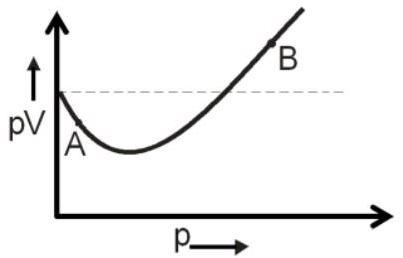
\includegraphics[max width=\textwidth, center]{2025_10_02_b63a859e04b52614bdbfg-1}
\end{enumerate}

What is the value of compressibility factor at point A?\\
(1) \(1-\frac{\mathrm{a}}{\text { RTV }}\)\\
(2) \(1+\frac{b}{V}\)\\
(3) \(1-\frac{b}{V}\)\\
(4) \(1+\frac{\mathrm{a}}{\text { RTV }}\)

Official Ans. by NTA (1)\\
Allen Ans. (1)\\
Sol. For 1 mole of real gas\\
\(\mathrm{PV}=\mathrm{ZRT}\)\\
from graph PV for real gas is less than PV for ideal gas at point A\\
\(\mathrm{Z}<1\)\\
\(\mathrm{Z}=1-\frac{\mathrm{a}}{\mathrm{V}_{\mathrm{m}} \mathrm{RT}}\)\\
32. The shortest wavelength of hydrogen atom in Lyman series is \(\lambda\). The longest wavelength in Balmer series of \(\mathrm{He}^{+}\)is\\
(1) \(\frac{5}{9 \lambda}\)\\
(2) \(\frac{9 \lambda}{5}\)\\
(3) \(\frac{36 \lambda}{5}\)\\
(4) \(\frac{5 \lambda}{9}\)

Official Ans. by NTA (2)\\
Allen Ans. (2)\\
Sol. For H: \(\frac{1}{\lambda}=\mathrm{R}_{\mathrm{H}} \times 1^{2}\left(\frac{1}{1^{2}}-\frac{1}{\infty^{2}}\right)\)\\
\(\frac{1}{\lambda_{\mathrm{He}^{+}}}=\mathrm{R}_{\mathrm{H}} \times 2^{2} \times\left(\frac{1}{4}-\frac{1}{9}\right)\)

From (1) \& (2) \(\frac{\lambda}{\lambda \mathrm{He}^{+}}=\frac{9}{5}\)\\
\(\lambda_{\mathrm{He}^{+}}=\lambda \times \frac{9}{5}\)\\
\(\lambda_{\mathrm{He}^{+}}=\frac{9 \lambda}{5}\)

\section*{TEST PAPER WITH SOLUTION}
\begin{enumerate}
  \setcounter{enumi}{32}
  \item Which of the following salt solutions would coagulate the colloid soloution formed when \(\mathrm{FeCl}_{3}\) is added to NaOH solution, at the fastest rate?\\
(1) 10 mL of \(0.2 \mathrm{~mol} \mathrm{dm}^{-3} \mathrm{AlCl}_{3}\)\\
(2) 10 mL of \(0.1 \mathrm{~mol} \mathrm{dm}^{-3} \mathrm{Na}_{2} \mathrm{SO}_{4}\)\\
(3) 10 mL of \(0.1 \mathrm{~mol} \mathrm{dm}^{-3} \mathrm{Ca}_{3}\left(\mathrm{PO}_{4}\right)_{2}\)\\
(4) 10 mL of \(0.15 \mathrm{~mol} \mathrm{dm}{ }^{-3} \mathrm{CaCl}_{2}\)
\end{enumerate}

Official Ans. by NTA (1)\\
Allen Ans. (1)\\
Sol. Sol. Formed is negatively charged solution, therefore \(\mathrm{Al}^{3+}\) has highest coagulating power\\
34. The bond dissociation energy is highest for\\
(1) \(\mathrm{Cl}_{2}\)\\
(2) \(\mathrm{I}_{2}\)\\
(3) \(\mathrm{Br}_{2}\)\\
(4) \(\mathrm{F}_{2}\)

Official Ans. by NTA (1)\\
Allen Ans. (1)\\
Sol. Bond energy of \(\mathrm{F}_{2}\) less than \(\mathrm{Cl}_{2}\) due to lone pair lone pair repulsions.\\
Bond energy order \(\mathrm{Cl}_{2}>\mathrm{Br}_{2}>\mathrm{F}_{2}>\mathrm{I}_{2}\)\\
35. The reaction representing the Mond process for metal refining is \(\_\_\_\_\)\\
(1) \(\mathrm{Ni}+4 \mathrm{CO} \xrightarrow{\Delta} \mathrm{Ni}(\mathrm{CO})_{4}\)\\
(2) \(2 \mathrm{~K}\left[\mathrm{Au}(\mathrm{CN})_{2}\right]+\mathrm{Zn} \xrightarrow{\Delta} \mathrm{K}_{2}\left[\mathrm{Zn}(\mathrm{CN})_{4}\right]+2 \mathrm{Au}\)\\
(3) \(\mathrm{Zr}+2 \mathrm{I}_{2} \xrightarrow{\Delta} \mathrm{Zr} \mathrm{I}_{4}\)\\
(4) \(\mathrm{ZnO}+\mathrm{C} \xrightarrow{\Delta} \mathrm{Zn}+\mathrm{CO}\)

Official Ans. by NTA (1)\\
Allen Ans. (1)\\
Sol. Mond's process uses:\\
\(\mathrm{Ni}+4 \mathrm{CO} \rightarrow\left[\mathrm{Ni}(\mathrm{CO})_{4}\right]\)\\
36. Which of the given compounds can enhance the efficiency of hydrogen storage tank?\\
(1) \(\mathrm{Li} / \mathrm{P}_{4}\)\\
(2) \(\mathrm{SiH}_{4}\)\\
(3) \(\mathrm{NaNi}_{5}\)\\
(4) Di-isobutylaluminium hydride

Official Ans. by NTA (3)\\
Allen Ans. (3)\\
Sol. Refer NCERT\\
37. The correct order of hydration enthalpies is\\
(A) \(\mathrm{K}^{+}\)\\
(B) \(\mathrm{Rb}^{+}\)\\
(C) \(\mathrm{Mg}^{2+}\)\\
(D) \(\mathrm{Cs}^{+}\)\\
(E) \(\mathrm{Ca}^{2+}\)

Choose the correct answer from the options given below:\\
(1) \(\mathrm{C}>\mathrm{A}>\mathrm{E}>\mathrm{B}>\mathrm{D}\)\\
(2) \(\mathrm{E}>\mathrm{C}>\mathrm{A}>\mathrm{B}>\mathrm{D}\)\\
(3) \(\mathrm{C}>\mathrm{E}>\mathrm{A}>\mathrm{D}>\mathrm{B}\)\\
(4) \(\mathrm{C}>\mathrm{E}>\mathrm{A}>\mathrm{B}>\mathrm{D}\)

Official Ans. by NTA (4)\\
Allen Ans. (4)\\
Sol. Hydration enthalpies:\\
(i) \(\mathrm{K}^{+}>\mathrm{Rb}^{+}>\mathrm{Cs}^{+}:(\mathrm{A})>(\mathrm{B})>(\mathrm{D})\)\\
(ii) \(\mathrm{Mg}^{+2}>\mathrm{Ca}^{+2}:(\mathrm{C})>(\mathrm{E})\)

Option (D)\\
(C) \(>\) (E) \(>\) (A) \(>\) (B) \(>\) (D)\\
38. The magnetic behaviour of \(\mathrm{Li}_{2} \mathrm{O}, \mathrm{Na}_{2} \mathrm{O}_{2}\) and \(\mathrm{KO}_{2}\), respectively, are\\
(1) diamagnetic, paramagnetic and diamagnetic\\
(2) paramagnetic, paramagnetic and diamagnetic\\
(3) paramagnetic, diamagnetic and paramagnetic\\
(4) diamagnetic, diamagnetic and paramagnetic

Official Ans. by NTA (4)\\
Allen Ans. (4)\\
Sol. \(\quad \mathrm{Li}_{2} \mathrm{O} \rightarrow \mathrm{O}^{2-} \rightarrow\) diamagnetic\\
\(\mathrm{Na}_{2} \mathrm{O}_{2} \rightarrow \mathrm{O}_{2}{ }^{2-} \rightarrow\) diamagnetic\\
\(\mathrm{KO}_{2} \rightarrow \mathrm{O}_{2}^{-} \rightarrow\) paramagnetic\\
39. "A" obtained by Ostwald's method involving air oxidation of \(\mathrm{NH}_{3}\), upon further air oxidation produces "B". "B" on hydration forms an oxoacid of Nitrogen along with evolution of "A". The oxoacid also produces "A" and gives positive brown ring test\\
(1) \(\mathrm{NO}_{2}, \mathrm{~N}_{2} \mathrm{O}_{5}\)\\
(2) \(\mathrm{NO}_{2}, \mathrm{~N}_{2} \mathrm{O}_{4}\)\\
(3) \(\mathrm{NO}, \mathrm{NO}_{2}\)\\
(4) \(\mathrm{N}_{2} \mathrm{O}_{3}, \mathrm{NO}_{2}\)

Official Ans. by NTA (3)\\
Allen Ans. (3)\\
Sol. \(4 \mathrm{NH}_{3}+5 \mathrm{O}_{2} \xrightarrow{\Delta} 4 \mathrm{NO}+6 \mathrm{H}_{2} \mathrm{O}\)\\
(A)\\
\(2 \mathrm{NO}+\mathrm{O}_{2} \longrightarrow 2 \mathrm{NO}_{2}\)\\
(B)\\
40. The standard electrode potential \(\left(\mathrm{M}^{3+} / \mathrm{M}^{2+}\right)\) for V , \(\mathrm{Cr}, \mathrm{Mn} \& \mathrm{Co}\) are \(-0.26 \mathrm{~V},-0.41 \mathrm{~V},+1.57 \mathrm{~V}\) and +1.97 V , respectively. The metal ions which can liberate \(\mathrm{H}_{2}\) from a dilute acid are\\
(1) \(\mathrm{V}^{2+}\) and \(\mathrm{Mn}^{2+}\)\\
(2) \(\mathrm{Cr}^{2+}\) and \(\mathrm{CO}^{2+}\)\\
(3) \(\mathrm{V}^{2+}\) and \(\mathrm{Cr}^{2+}\)\\
(4) \(\mathrm{Mn}^{2+}\) and \(\mathrm{Co}^{2+}\)

Official Ans. by NTA (3)\\
Allen Ans. (3)\\
Sol. Metal cation with ( - ) value of reduction potential \(\left(\mathrm{M}^{+3} / \mathrm{M}^{+2}\right)\) or with \((+)\) value of oxidation potential ( \(\mathrm{M}^{+2} / \mathrm{M}^{+3}\) ) will liberate \(\mathrm{H}_{2}\)\\
Therefore they will reduce \(\mathrm{H}^{+}\)\\
i. \(\mathrm{eV}^{+2}\) and \(\mathrm{Cr}^{+2}\)\\
41. Correct statement about smog is\\
(1) \(\mathrm{NO}_{2}\) is present in classical smog\\
(2) Both \(\mathrm{NO}_{2}\) and \(\mathrm{SO}_{2}\) are present in classical smog\\
(3) Photochemical smog has high concentration of oxidizing agents\\
(4) Classical smog also has high concentration of oxidizing agents\\
Official Ans. by NTA (3)\\
Allen Ans. (3)\\
Sol. Photochemical smog has high concentration of oxidising agents\\
\(\mathrm{NO}_{2}\) is produced from NO and \(\mathrm{O}_{3}\) in the presence of sunlight\\
Classical smog contain smoke, fog and \(\mathrm{SO}_{2}\) and it is known as reducing smog, as chemically it is reducing mixture\\
42. Chiral complex from the following is :

Here en \(=\) ethylene diamine\\
(1) cis \(-\left[\mathrm{PtCl}_{2}(\mathrm{en})_{2}\right]^{2+}\)\\
(2) trans \(-\left[\mathrm{PtCl}_{2}(\mathrm{en})_{2}\right]^{2+}\)\\
(3) cis - \(\left[\mathrm{PtCl}_{2}\left(\mathrm{NH}_{3}\right)_{2}\right]\)\\
(4) trans \(-\left[\mathrm{Co}\left(\mathrm{NH}_{3}\right)_{4} \mathrm{Cl}_{2}\right]^{+}\)

Official Ans. by NTA (1)\\
Allen Ans. (1)\\
Sol.\\
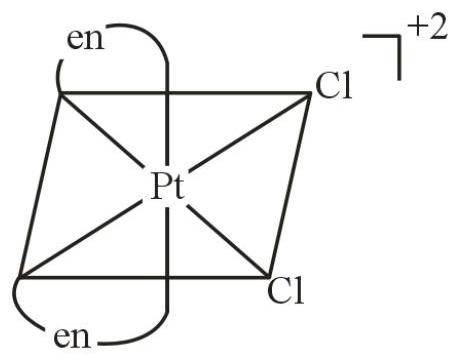
\includegraphics[max width=\textwidth, center]{2025_10_02_b63a859e04b52614bdbfg-2}\\
this is chiral complex form\\
43. Identify the correct order for the given property for following compounds\\
(A) Boiling Point:\\
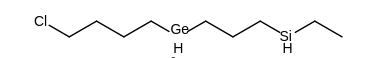
\includegraphics{smile-7f501c0d5913705987ed7177d6b9de20035962b9}\\
(B) Density:\\
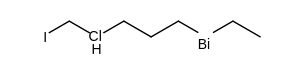
\includegraphics{smile-73fda6bef08487dc922f226df2dd2d00f7335c85}\\
(C) Boiling Point:\\
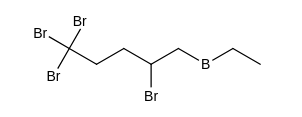
\includegraphics{smile-c15ba54d0836d1d3988a03ac444b2ecb5a8d3d71}\\
(D) Density:\\
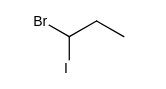
\includegraphics{smile-b941bdf20b3a43ab9f28192bb25beaeefc373d5d}\\
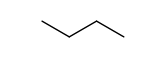
\includegraphics{smile-884c72ed68930c4eab8496f2e20c1081595dfda6}\\
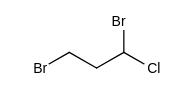
\includegraphics{smile-e15bfce31e8f18499c04dadd8f2134503fa76faf}\\
(E) Boiling Point:\\
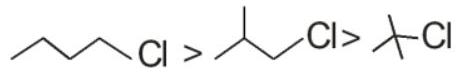
\includegraphics[max width=\textwidth, center]{2025_10_02_b63a859e04b52614bdbfg-3(1)}

Choose the correct answer from the option given below :-\\
(1) (B), (C) and (D) only\\
(2) (A), (C) and (E) only\\
(3) (A), (C) and (D) only\\
(4) (A), (B) and (E) only

Official Ans. by NTA (2)\\
Allen Ans. (2)\\
Sol. Boiling point of alkyl halide increases with increase in size, mass of halogen atom and size of alkyl group

Boiling point of isomeric alkyl halide decreases with increase in branching\\
Density increases with increase in atomic mass of halogen atom\\
44. The increasing order of \(\mathrm{pK}_{\mathrm{a}}\) for the following phenols is\\
(1) 2, 4-Dinitrophenol\\
(2) 4 - Nitrophenol\\
(3) 2, 4, 5-Trimethylphenol\\
(4) Phenol\\
(5) 3-Chlorophenol

\section*{Official Ans. by NTA (2)}
Allen Ans. (2)\\
Sol. Order of acidity for following phenol is\\
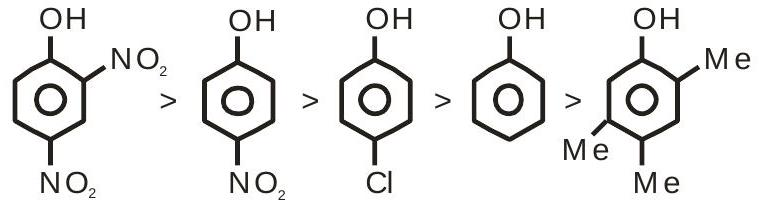
\includegraphics[max width=\textwidth, center]{2025_10_02_b63a859e04b52614bdbfg-3(2)}

\begin{itemize}
  \item M and - I increases acidity
\end{itemize}

\begin{itemize}
  \item M and + I decreases acidity
\end{itemize}

\begin{enumerate}
  \setcounter{enumi}{44}
  \item Match List I with List II.
\end{enumerate}

\section*{Sol. Reactions}
(A) Hoffmann degradation\\
(B) Clemenson reduction\\
(C) Cannizaro reaction\\
(D) Reimer-Tiemann reaction

\section*{Reagent used}
\(\mathrm{Br}_{2} / \mathrm{NaOH}\)\\
\(\mathrm{Zn}-\mathrm{Hg} / \mathrm{HCl}\)\\
conc. \(\mathrm{KOH} / \Delta\)\\
\(\mathrm{CHCl}_{3}\), \(\mathrm{NaOH} / \mathrm{H}_{3} \mathrm{O}^{+}\)

\begin{center}
\begin{tabular}{|l|l|}
\hline
List-I & List-II \\
\hline
Reaction & Reagents \\
\hline
(A) Hoffmann Degradation & (I) Conc. \(\mathrm{KOH}, \Delta\) \\
\hline
(B) Clemenson reduction & (II) \(\mathrm{CHCl}_{3}, \mathrm{NaOH} / \mathrm{H}_{3} \mathrm{O}^{+}\) \\
\hline
(C) Cannizaro reaction & (III) \(\mathrm{Br}_{2}, \mathrm{NaOH}\) \\
\hline
(D) Reimer-Tiemann reaction & (IV) \(\mathrm{Zn}-\mathrm{Hg} / \mathrm{HCl}\) \\
\hline
\end{tabular}
\end{center}

(1) (A) - III, (B) - IV, (C) - II, (D) - I\\
(2) (A) - II, (B) - IV, (C) - I, (D) - III\\
(3) (A) - III, (B) - IV, (C) - I, (D) - II\\
(4) (A) - II, (B) - I, (C) - III, (D) - IV

Official Ans. by NTA (3)\\
Allen Ans. (3)\\
46. The major product ' P ' for the following sequence of reactions is:\\
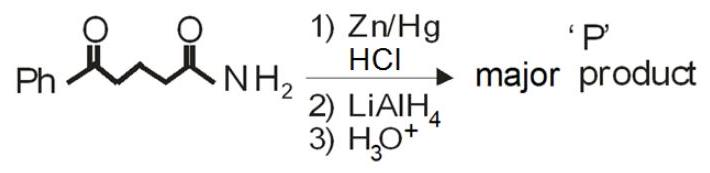
\includegraphics[max width=\textwidth, center]{2025_10_02_b63a859e04b52614bdbfg-3(3)}\\
(1)\\
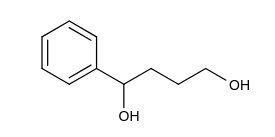
\includegraphics{smile-541c62fc928ead77bbc693a77c8a92dc3145bc5d}\\
(2)\\
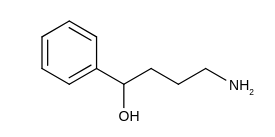
\includegraphics{smile-25a17a5c6b296987ecbae8c9827c4d2138fe807c}\\
(3)\\
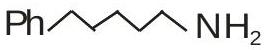
\includegraphics[max width=\textwidth, center]{2025_10_02_b63a859e04b52614bdbfg-3}\\
(4)\\
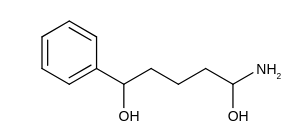
\includegraphics{smile-a605706018c7e5d1da75b64be99138593794a9e6}

Official Ans. by NTA (3)\\
Allen Ans. (3)\\
Sol.\\
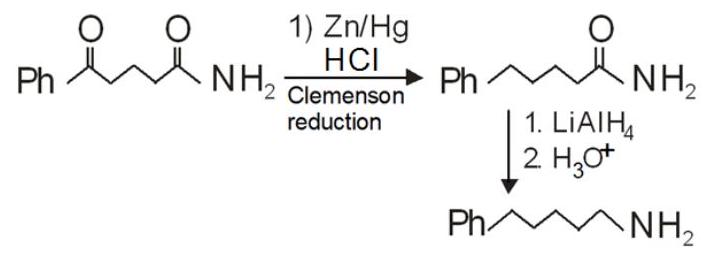
\includegraphics[max width=\textwidth, center]{2025_10_02_b63a859e04b52614bdbfg-3(4)}\\
47. During the borax bead test with \(\mathrm{CuSO}_{4}\), a blue green colour of the bead was observed in oxidising flame due to the formation of\\
(1) \(\mathrm{Cu}_{3} \mathrm{~B}_{2}\)\\
(2) Cu\\
(3) \(\mathrm{Cu}\left(\mathrm{BO}_{2}\right)_{2}\)\\
(4) CuO

\section*{Official Ans. by NTA (3)}
\section*{Allen Ans. (3)}
Sol. Blue green colour is due to formation of \(\mathrm{Cu}\left(\mathrm{BO}_{2}\right)_{2}\)

\[
\begin{aligned}
& \mathrm{CuSO}_{4} \xrightarrow{\Delta} \mathrm{CuO}+\mathrm{SO}_{3} \\
& \mathrm{CuO}+\mathrm{B}_{2} \mathrm{O}_{3} \rightarrow \mathrm{Cu}\left(\mathrm{BO}_{2}\right)_{2}
\end{aligned}
\]

\begin{enumerate}
  \setcounter{enumi}{47}
  \item Match List I with List II
\end{enumerate}

\begin{center}
\begin{tabular}{|l|l|}
\hline
List I & List II \\
\hline
Antimicrobials & Names \\
\hline
(A) Narrow Spectrum Antibiotic & (I) Furacin \\
\hline
(B) Antiseptic & (II) Sulphur dioxide \\
\hline
(C) Disinfectants & (III) Penicillin-G \\
\hline
(D) Broad spectrum antibiotic & (IV) Chloramphenicol \\
\hline
\end{tabular}
\end{center}

(1) (A) - III, (B) - I, (C) - II, (D) - IV\\
(2) (A) - I, (B) - II, (C) - IV, (D) - III\\
(3) (A) - II, (B) - I, (C) - IV, (D) - III\\
(4) (A) - III, (B) - I, (C) - IV, (D) - II

Official Ans. by NTA (1)\\
Allen Ans. (1)\\
Sol. (A) Narrow spectrum antibiotic - penicillin-G\\
(B) Antiseptic - Furacine\\
(C) Disinfectants - sulphur dioxide\\
(D) Broad spectrum antisiotics - chloramphenicol\\
49. Number of cyclic tripeptides formed with 2 amino acids \(A\) and \(B\) is:\\
(1) 2\\
(2) 3\\
(3) 5\\
(4) 4

\section*{Official Ans. by NTA (4)}
\section*{Allen Ans. (4)}
Sol. Two amino acid are\\
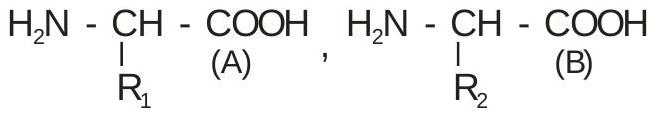
\includegraphics[max width=\textwidth, center]{2025_10_02_b63a859e04b52614bdbfg-4}

Tripeptide are formed from three amino acids\\
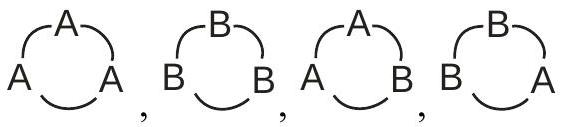
\includegraphics[max width=\textwidth, center]{2025_10_02_b63a859e04b52614bdbfg-4(1)}\\
50. Compound that will give positive Lassaigne's test for both nitrogen and halogen is\\
(1) \(\mathrm{N}_{2} \mathrm{H}_{4} \cdot \mathrm{HCl}\)\\
(2) \(\mathrm{CH}_{3} \mathrm{NH}_{2} \cdot \mathrm{HCl}\)\\
(3) \(\mathrm{NH}_{4} \mathrm{Cl}\)\\
(4) \(\mathrm{NH}_{2} \mathrm{OH} . \mathrm{HCl}\)

Official Ans. by NTA (2)\\
Allen Ans. (2)\\
Sol. \(\mathrm{CH}_{3} \mathrm{NH}_{2} . \mathrm{HCl} \xrightarrow[\text { fusion }]{\mathrm{Na}} \mathrm{NaCN}\) and NaCl\\
NaCN gives + ve test for nitrogen and\\
NaCl gives +ve test for halogen

\section*{SECTION-B}
\begin{enumerate}
  \setcounter{enumi}{50}
  \item Millimoles of calcium hydroxyide required to produce 100 mL of the aqueous solution of pH 12 is \(x \times 10^{-1}\). The value of \(x\) is \(\_\_\_\_\) (Nearest integer). Assume complete dissociation.\\
Official Ans. by NTA (5)\\
Allen Ans. (5)\\
Sol. \(\because \mathrm{pH}=12\)\\
\(\therefore\left[\mathrm{H}^{+}\right]=10^{-12} \mathrm{M}\)\\
\(\therefore\left[\mathrm{OH}^{-}\right]=10^{-2} \mathrm{M}\)\\
\(\therefore\left[\mathrm{Ca}(\mathrm{OH})_{2}\right]=5 \times 10^{-3} \mathrm{M}\)\\
\(5 \times 10^{-3}=\frac{\text { milli moles of } \mathrm{Ca}(\mathrm{OH})_{2}}{100 \mathrm{~mL}}\)\\
milli moles of \(\mathrm{Ca}(\mathrm{OH})_{2}=5 \times 10^{-1}\)\\
Ans. \(=5\)
  \item The number of molecules or ions from the following, which do not have odd number of electrons are \(\_\_\_\_\) .\\
(A) \(\mathrm{NO}_{2}\)\\
(B) \(\mathrm{ICl}_{4}^{-}\)\\
(C) \(\mathrm{BrF}_{3}\)\\
(D) \(\mathrm{ClO}_{2}\)\\
(E) \(\mathrm{NO}_{2}^{+}\)\\
(F) NO
\end{enumerate}

Official Ans. by NTA (3)\\
Allen Ans. (3)\\
Sol. \(\mathrm{ICl}_{4}{ }^{-}, \mathrm{BrF}_{3}\) and \(\mathrm{NO}_{2}{ }^{+}\)do not have odd number of \(\mathrm{e}^{-}\)\\
53. Consider the following reaction approaching equilibrium at \(27^{\circ} \mathrm{C}\) and 1 atm pressure\\
\(\mathrm{A}+\mathrm{B} \underset{\mathrm{K}_{\mathrm{r}}=10^{2}}{\stackrel{\mathrm{~K}_{\mathrm{f}}=10^{3}}{\rightleftharpoons}} \mathrm{C}+\mathrm{D}\)\\
The standard Gibb's energy change ( \(\Delta_{\mathrm{r}} \mathrm{G}^{\circ}\) ) at \(27^{\circ} \mathrm{C}\) is ( - ) \(\_\_\_\_\) \(\mathrm{kJ} \mathrm{mol}^{-1}\)\\
(Nearest integer).\\
(Given : \(\mathrm{R}=8.3 \mathrm{~J} \mathrm{~K}^{-1} \mathrm{~mol}^{-1}\) and \(\ln 10=2.3\) )\\
Official Ans. by NTA (6)\\
Allen Ans. (6)\\
Sol. \(\because \Delta \mathrm{G}^{\circ}=-\mathrm{RT} \ln \mathrm{K}_{\mathrm{eq}}\)\\
and \(\mathrm{K}_{\mathrm{eq}}=\frac{\mathrm{K}_{\mathrm{f}}}{\mathrm{K}_{\mathrm{b}}}\)\\
\(\therefore \mathrm{K}_{\text {eq }}=\frac{10^{3}}{10^{2}}=10\)\\
\(\therefore \Delta \mathrm{G}=-\mathrm{RT} \ln 10\)\\
\(\Rightarrow-(8.3 \times 300 \times 2.3)=-5.7 \mathrm{~kJ} \mathrm{~mole}^{-1} \approx 6 \mathrm{~kJ}\) mole \(^{-1}\) (nearest integer)\\
Ans \(=6\)\\
54. Solid Lead nitrate is dissolved in 1 litre of water. The solution was found to boil at \(100.15^{\circ} \mathrm{C}\). When 0.2 mol of NaCl is added to the resulting solution, it was observed that the solution froze at \(-0.8^{\circ} \mathrm{C}\). The solutbility product of \(\mathrm{PbCl}_{2}\) formed is \(\_\_\_\_\) \(\times 10^{-6}\) at 298 K . (Nearest integer)\\
Given : \(\mathrm{K}_{\mathrm{b}}=0.5 \mathrm{~K} \mathrm{~kg} \mathrm{~mol}^{-1}\) and \(\mathrm{K}_{\mathrm{f}}=1.8 \mathrm{~kg} \mathrm{~mol}^{-1}\). Assume molality to be equal to molarity in all cases.\\
Official Ans. by NTA (13)\\
Allen Ans. (13)\\
Sol. Let a mole \(\mathrm{Pb}\left(\mathrm{NO}_{3}\right)_{2}\) be added\\
\(\mathrm{Pb}\left(\mathrm{NO}_{3}\right)_{2} \rightarrow \mathrm{~Pb}^{2+}+2 \mathrm{NO}_{3}^{-}\)

\[
\begin{array}{lcc}
\mathrm{a} & \mathrm{a} \quad 2 \mathrm{a} \\
\Delta \mathrm{~T}_{\mathrm{b}}=0.15=0.5[3 \mathrm{a}] \Rightarrow \mathrm{a}=0.1 \\
& \mathrm{~Pb}_{(\mathrm{aq})}^{2+}+ & 2 \mathrm{Cl}_{(\mathrm{aq})}^{-} \rightarrow \mathrm{PbCl}_{2}(\mathrm{~s}) \\
\mathrm{t}=0 & 0.1 & 0.2 \\
\mathrm{t}=\infty & (0.1-\mathrm{x}) & (0.2-2 \mathrm{x})
\end{array}
\]

In final solution\\
\(\Delta \mathrm{T}_{\mathrm{f}}=0.8=1.8\left[\frac{0.3-3 \mathrm{x}+0.2+0.2}{1}\right]\)\\
\(\Rightarrow \mathrm{x}=\frac{2.3}{27}\)\\
\(\Rightarrow \mathrm{K}_{\mathrm{sp}}=\left(0.1-\frac{2.3}{27}\right)\left(0.2-\frac{4.6}{27}\right)^{2}=13 \times 10^{-6}\)\\
55. Water decomposes at 2300 K\\
\(\mathrm{H}_{2} \mathrm{O}(\mathrm{g}) \rightarrow \mathrm{H}_{2}(\mathrm{~g})+\frac{1}{2} \mathrm{O}_{2}(\mathrm{~g})\)\\
The percent of water decomposing at 2300 K and 1 bar is \(\_\_\_\_\) (Nearest integer).

Equilibrium constant for the reaction is \(2 \times 10^{-3}\) at 2300 K

Official Ans. by NTA (2)\\
Allen Ans. (2)\\
Sol. \(\mathrm{H}_{2} \mathrm{O}(\mathrm{g}) \rightleftharpoons \mathrm{H}_{2}(\mathrm{~g})+\frac{1}{2} \mathrm{O}_{2}(\mathrm{~g})\)\\
\(\mathrm{P}_{0}[1-\alpha] \quad \mathrm{P}_{0} \alpha \quad \frac{\mathrm{P}_{0} \alpha}{2} \quad\) partial pr. at eq.\\
\(\mathrm{P}_{0}\left[1+\frac{\alpha}{2}\right]=1\)\\
\(\mathrm{K}_{\mathrm{p}}=\frac{\left(\mathrm{P}_{\mathrm{H}_{2}}\right)\left(\mathrm{P}_{\mathrm{O}_{2}}\right)^{1 / 2}}{\mathrm{P}_{\mathrm{H}_{2} \mathrm{O}}}\)\\
\(\frac{\left(\mathrm{P}_{0} \alpha\right)\left(\frac{\mathrm{P}_{0} \alpha}{2}\right)^{1 / 2}}{\mathrm{P}_{0}[1-\alpha]}=2 \times 10^{-3}\)\\
since \(\alpha\) is negligible w.r.t 1 so \(\mathrm{P}_{0}=1\) and \(1-\alpha \approx 1\)\\
\(\frac{\alpha \sqrt{\alpha}}{\sqrt{2}}=2 \times 10^{-3}\)\\
\(\alpha^{3 / 2}=2^{3 / 2} \times 10^{-3}\)\\
\(\alpha=2^{3 / 2 \times 2 / 3} \times 10^{-3 \times 2 / 3}\)\\
\(\alpha=2 \times 10^{-2} \quad \% \alpha=2 \%\)\\
56. Following figure shows dependence of molar conductance of two electrolytes on concentration. \(\Lambda \stackrel{0}{\mathrm{~m}}\) is the limiting molar conductivity.\\
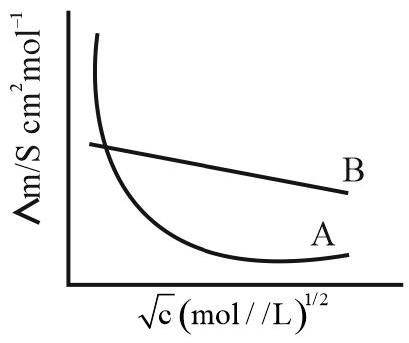
\includegraphics[max width=\textwidth, center]{2025_10_02_b63a859e04b52614bdbfg-5}

The number of Incorrect statement(s) from the following is \(\_\_\_\_\)\\
(A) \(\Lambda \mathrm{m}\) for electrolyte A is obtained by extrapolation\\
(B) For electrolyte \(B\), vx \(\Lambda \mathrm{m} v s \sqrt{\mathrm{c}}\) graph is a 0 straight line with intercept equal to \(\Lambda \mathrm{m}\)\\
(C) At infinite dilution, the value of degree of dissociation approach zero for electrolyte B.\\
(D) \(\Lambda \stackrel{0}{\mathrm{~m}}\) for any electrolyte A or B can be calculated using \(\lambda^{\circ}\) for individual ions.\\
Official Ans. by NTA (2)\\
Allen Ans. (2)\\
Sol. Statement (A) and Statement (C) are incorrect\\
57. For certain chemical reaction \(\mathrm{X} \rightarrow \mathrm{Y}\), the rate of formation of product is plotted against the time as shown in the figure. The number of Correct statement/s from the following is \(\_\_\_\_\)\\
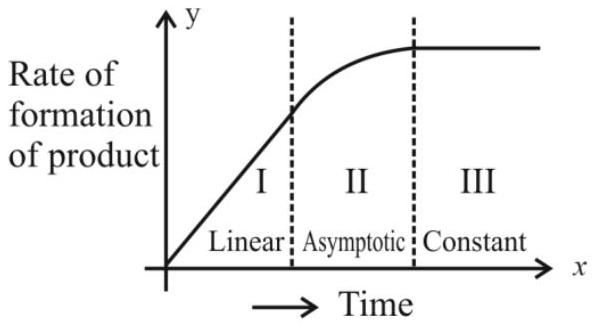
\includegraphics[max width=\textwidth, center]{2025_10_02_b63a859e04b52614bdbfg-6}\\
(A) Over all order of this reaction is one\\
(B) Order of this reaction can't be determined\\
(C) In region-I and III, the reaction is of first and zero order respectively\\
(D) In region-II, the reaction is of first order\\
(E) In region-II, the order of reaction is in the range of 0.1 to 0.9 .\\
Official Ans. by NTA (2)\\
Allen Ans. (1)\\
Sol. Only option (B) is correct as order cannot be determined\\
58. The sum of bridging carbonyls in \(\mathrm{W}(\mathrm{CO})_{6}\) and \(\mathrm{Mn}_{2} (\mathrm{CO})_{10}\) is \(\_\_\_\_\) .

\section*{Official Ans. by NTA (0)}
Allen Ans. (0)\\
Sol.\\
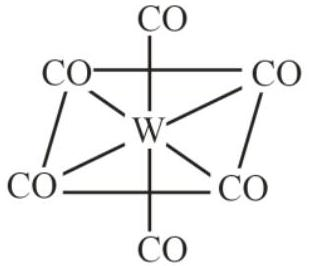
\includegraphics[max width=\textwidth, center]{2025_10_02_b63a859e04b52614bdbfg-6(2)}\\
\(\left[(\mathrm{CO})_{5} \mathrm{Mn}-\mathrm{Mn}(\mathrm{CO})_{5}\right]\)\\
59. Following chromatogram was developed by adsorption of compound ' A ' on a 6 cm TLC glass plate. Retardation factor of the compound ' A ' is\\
\(\_\_\_\_\) \(\times 10^{-1}\).\\
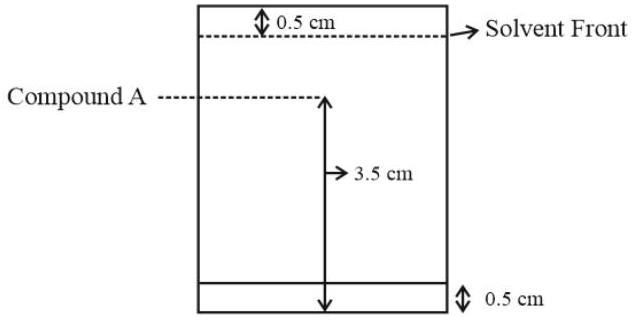
\includegraphics[max width=\textwidth, center]{2025_10_02_b63a859e04b52614bdbfg-6(1)}

Official Ans. by NTA (6)\\
Allen Ans. (6)\\
Sol. \(\quad \mathrm{R}_{\mathrm{f}}=\frac{\text { Distance moved by the substance from base line }}{\text { Distance moved by the solvent from base line }}\)\\
\(=\frac{3.0 \mathrm{~cm}}{5.0 \mathrm{~cm}}=0.6\) or \(6 \times 10^{-1}\)\\
60. 17 mg of a hydrocarbon (M.F. \(\mathrm{C}_{10} \mathrm{H}_{16}\) ) takes up 8.40 mL of the \(\mathrm{H}_{2}\) gas measured at \(0^{\circ} \mathrm{C}\) and 760 mm of Hg . Ozonolysis of the same hydrocarbon yields\\
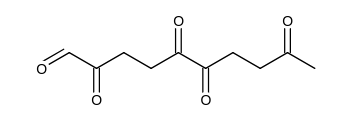
\includegraphics{smile-a811cd5fb14caa3c835ca8a8c6e8620bac0b6a4c}

The number of double bond/s present in the hydrocarbon is \(\_\_\_\_\) .\\
Official Ans. by NTA (3)\\
Allen Ans. (3)\\
Sol. Moles of hydrocarbon \(=\frac{17 \times 10^{-3}}{136}=1.25 \times 10^{-4}\)\\
Mole of \(\mathrm{H}_{2}\) gas\\
\(\Rightarrow 1 \times \frac{8.40}{1000}=\mathrm{n} \times 0.0821 \times 273\)\\
\(\Rightarrow \mathrm{n}=3.75 \times 10^{-4}\)\\
Hydrogen molecule used for 1 molecule of hydrocarbon is 3\\
\(=\frac{3.75 \times 10^{-4}}{1.25 \times 10^{-4}}=3\)


\end{document}